\section{Progettazione Logica}

\subsection{Modelli logici per il data mart}
Prendere gli schemi di fatto e tradurli in una implementazione coerente con il modello scelto (ROLAP o MOLAP). Esistono due tipi di schemi standard che si usano quando si implementa un cubo su una piattaforma ROLAP. Il principale è lo schema a stella ed è un modo classico per rappresentare un contenuto multidimensionale su un DB relazionale. Uno schema a stella è composto da:
\begin{itemize}
	\item 
	\textbf{Dimension Table}: una per ogni dimensione del cubo, in cui si ha una chiave primaria (un surrogato) e dentro si hanno tutti gli attributi della gerarchia
	\item
	\textbf{Fact table}: importa al suo interno Foreign Key prese da tutte le DT. Tutte le FK insieme formano la chiave primaria e in più si trovano le misure
\end{itemize}

\textbf{Considerazioni}

Le DT sono completamente denormalizzate, non sono in terza forma normale e non si hanno problemi di sparsità in quanto vengono memorizzzate soltanto le tuple corrispondenti a punti dello spazio multidimensionale per cui esistono eventi. 
\begin{figure}[H]
	\centering
	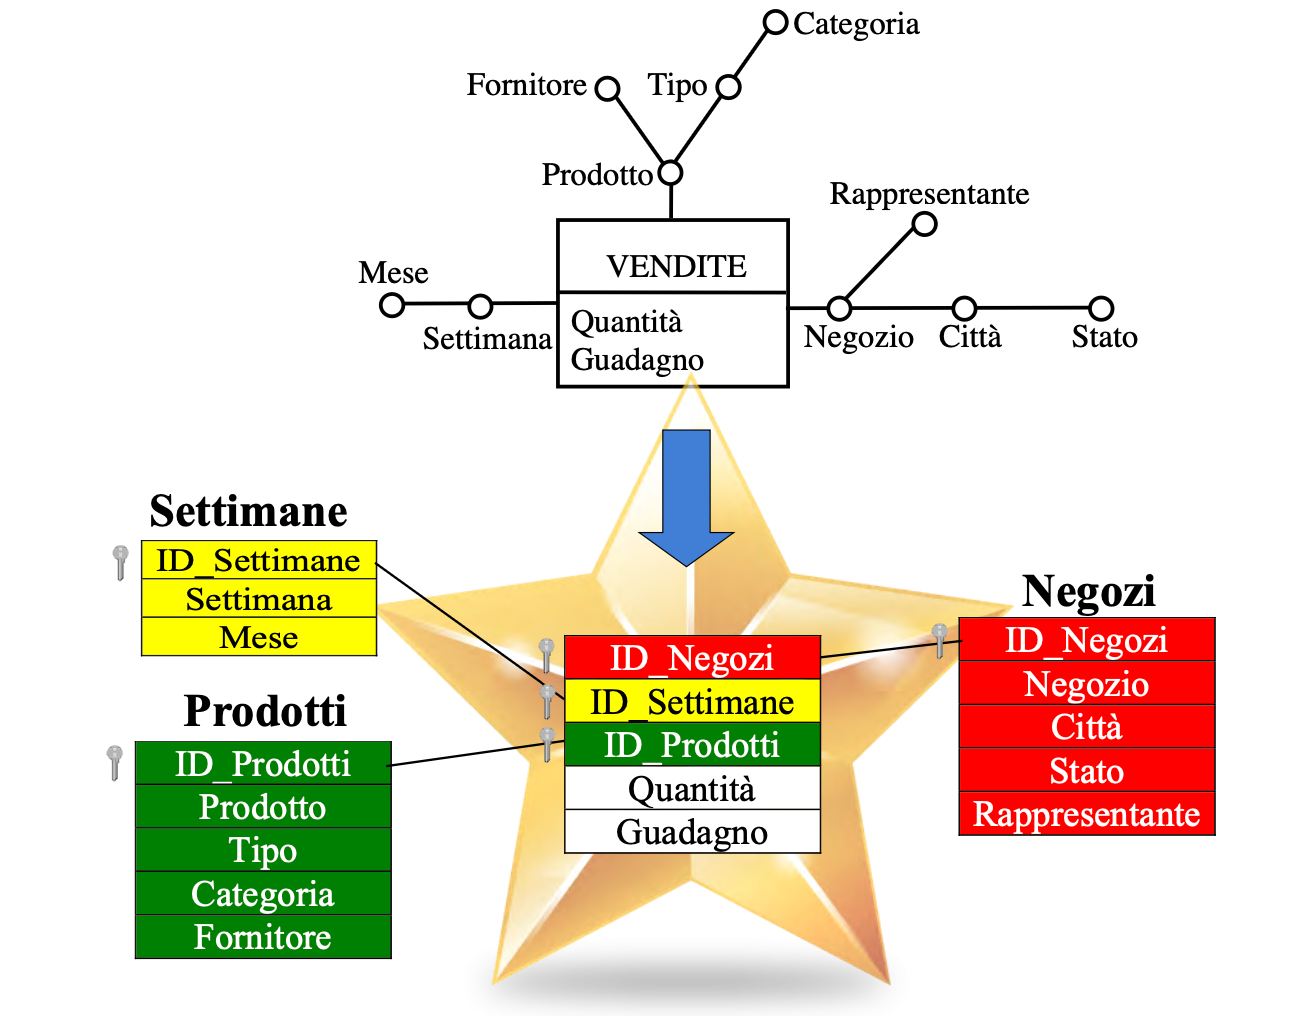
\includegraphics[width=0.6\linewidth]{img/stella}
	\caption{Schema a Stella}
	\label{fig:stella}
\end{figure}
Il secondo tipo di schema che si usa si chiama snowflake, il quale è una variante dello schema a stella, la cui caratteristica è che le DT vengono completamente o parzialmente normalizzate. 

\textbf{Considerazioni}

\begin{itemize}
	\item
	Lo spazio richiesto si riduce in linea di principio perché normalizzando elimino le ridondanze, ma è anche vero che ho aggiunto dei surrogati che nello schema a stella non si hanno
	\item 
	L’esecuzione di interrogazioni che coinvolgono solo gli attributi contenuti nella fact table e nelle dimension table primarie è avvantaggiata
	\item 
	Il tempo di esecuzione delle interrogazioni che coinvolgono attributi delle dimension table secondarie aumenta
\end{itemize}
\begin{figure}[H]
	\centering
	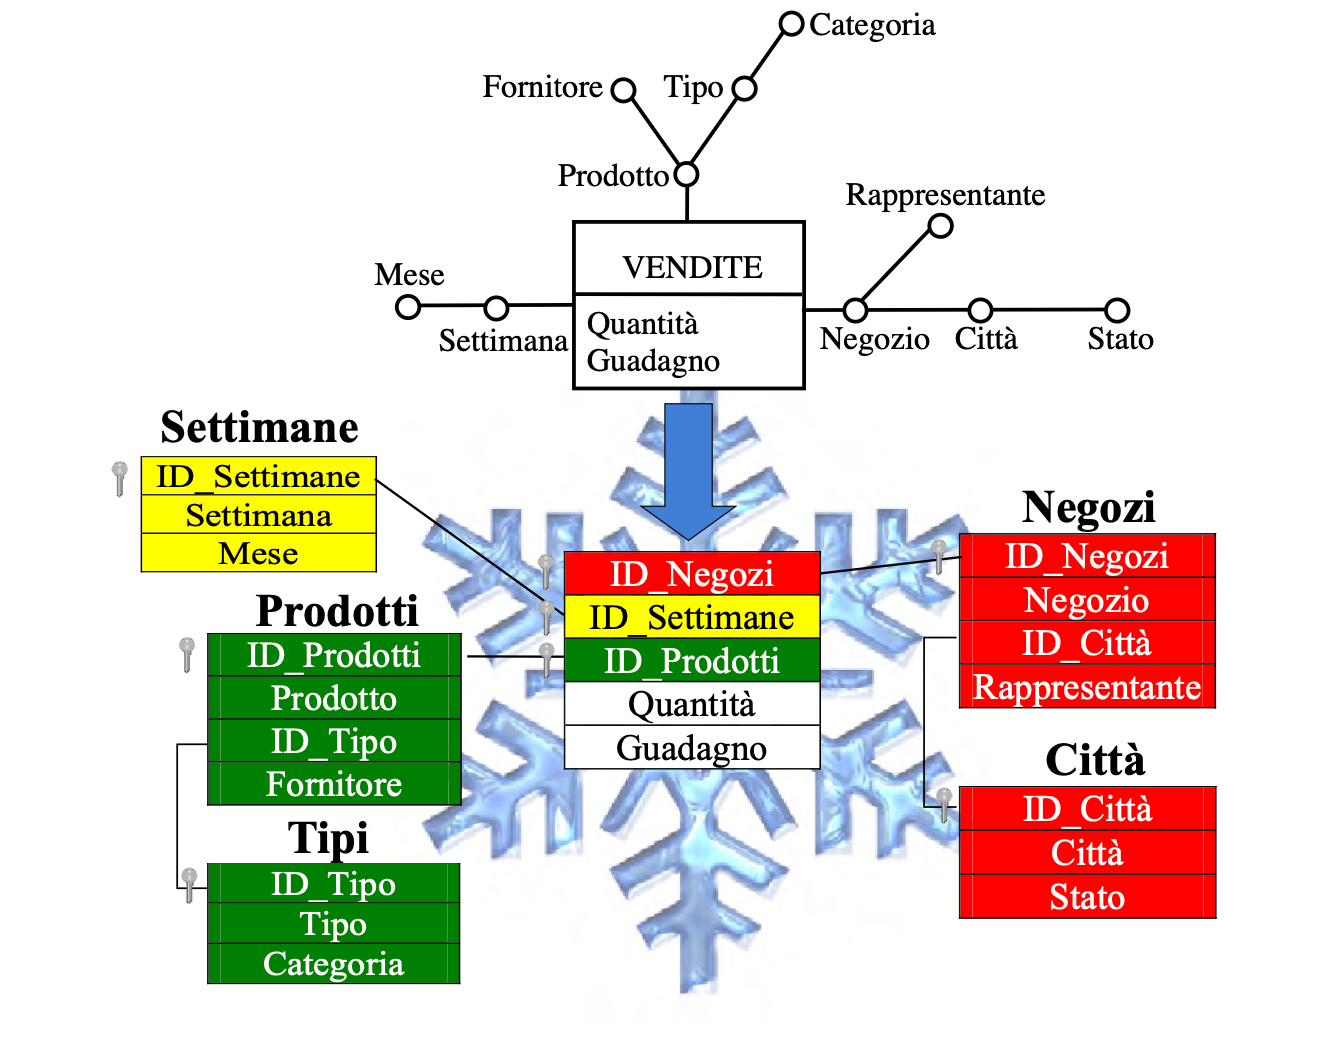
\includegraphics[width=0.6\linewidth]{img/snowflake}
	\caption{Snowflake}
	\label{fig:snowflake}
\end{figure}

\subsection{Le viste}
La tecnica più usata in ambito ROLAP per ottimizzare le prestazioni è la cosiddetta materializzazione delle viste, in quando ci saranno query frequentemente richieste, allora per ottimizzare queste query materializzo, cioè creo fisicamente nel DB delle viste (ossia tabelle) che memorizzano esattamente il risultato della query. 

Nelle viste normalmente non si mettono dei predicati di selezioni, ma tutti gli eventi aggregati in un certo modo. La vista viene denotata in base ad un certo group-by set. 

L’utilità nel creare una vista, non è solo limitata alle query che hanno quel group-by ma anche a query che sono ulteriormente aggregate. Questo ragionamento viene supportato dal reticolo, il quale è una struttura algebrica.
\begin{figure}[H]
	\centering
	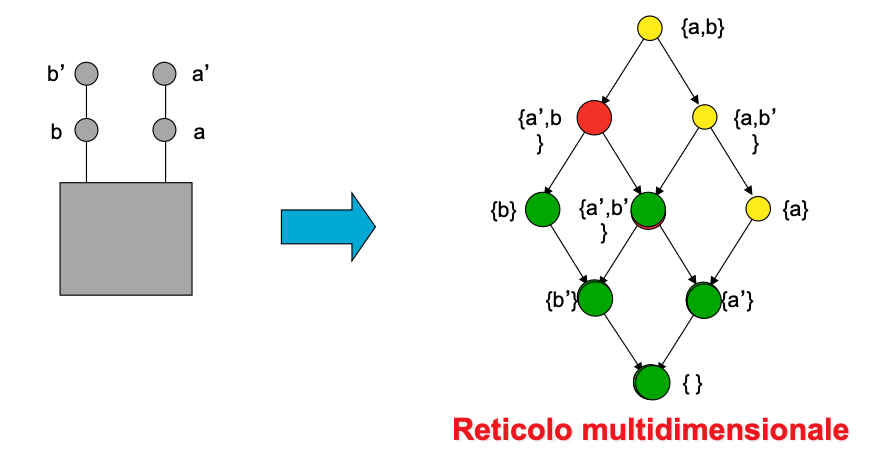
\includegraphics[width=0.6\linewidth]{img/reticolo}
	\caption{Reticolo multidimensionale}
	\label{fig:reticolo}
\end{figure}

Supponiamo di avere il DFM in figura \ref{fig:reticolo} con due dimensioni e due micro-gerarchie. A destra troviamo il reticolo multidimensionale completo, cioè si ha dentro un nodo per ogni possibile group-by di quel DFM. Sono tutti disposti in questa struttura, in cui si ha sempre un top e un bottom. Il primo è quello più fine, quello che corrisponde alle dimensioni. Il bottom è il group-by vuoto, aggrego tutto in un mega evento secondario. Le frecce indicano che da un dato aggregato facendo un ulteriore aggregazione posso calcolare un dato che è ancora più aggregato. Se scelgo la vista più in alto possibile, sto dicendo che questa la uso spesso, in quanto mi copre più query, ma dovrei aggregare sempre. Avendola scelta così in alto, la vista è grande, cioè quanto la fact table primaria e mi porta ad un incremento delle prestazioni trascurabile. Se la scegliessi in basso migliora ma per poche query. In realtà la materializzazione delle viste deve essere fatta sul carico di lavoro. 
\subsubsection{Schemi relazioniali e viste}
Adottando lo snowflake schema è possibile memorizzare in fact table separate dati appartenenti a diversi group-by set.


Nei motori multidimensionali vi è un componente, l’aggregate navigator, che in maniera trasparente per l’utente decide quale vista utilizzare per ciascuna query. Ha accesso ai metadati, sa come sono fatte le gerarchie, conosce le dipendenze funzionali, sa quali sono le viste che gli utenti hanno creato. Ha il compito di capire su quale fact table quella query è eseguibile.

\subsection{Progettazione logica}
Include l’insieme dei passi che, a partire dallo schema concettuale, permettono di determinare lo schema logico del data mart. In input ho lo schema concettuale, conosco il carico di lavoro e il volume dati, e in output, devo ottenere lo schema logico. I principi basati per fare questa traduzione non sono gli stessi utilizzati per i DB operazionali. Gli step da fare sono:
\begin{enumerate}
	\item
	Scelta dello schema logico da utilizzare (schema a stella o snowflake) 
	\item 
	Traduzione degli schemi concettuali
	\item 
	Scelte delle viste da materializzare
	\item 
	Applicazione di altre forme di ottimizzazione
\end{enumerate}

\textbf{Star vs Snowflake}

Primo ragionamento che si può fare è legato alla cardinalità di dominio, cioè al numero di valori distinti per ogni attributo. L’unico caso in cui si utilizza snowflake è quando si ha una gerarchia condivisa. 

La regola di base per la traduzione di uno schema di fatto in schema a stella prevede di: 
\begin{itemize}
	\item
	Creare una fact table contenente tutte le misure e gli attributi descrittivi direttamente collegati con il fatto
	\item 
	Per ogni gerarchia, creare una dimension table che ne contiene tutti gli attributi.
\end{itemize}
In aggiunta a questa semplice regola, la corretta traduzione di uno schema di fatto richiede una trattazione approfondita dei costrutti avanzati del DFM:
\begin{itemize}
	\item 
	\textbf{Attributi descrittivi}: finisce nella stessa DT nella quale finisce suo padre
	\item
	\textbf{Archi opzionali}: tutti gli attributi a valle dell’arco opzionale finiscono nella stessa DT del padre.
	\item 
	\textbf{Gerarchia condivisa}: se è su una dimensione, allora si crea un unico DT e la si usa più volte. Se invece la condivisione è da qualche altra parte e non sulla dimensione allora ho due scelte: snowflaking o ripetere gi attributi in entrambe le tabelle. 
	\item 
	\textbf{Convergenza}: si includono nella stessa DT dei loro attributi padri
	\item 
	\textbf{Gerarchie incomplete}: basta sapere che dal punto di vista dello schema non ci sono impatti particolari
	\item 
	\textbf{Scelta delle viste}: è un compito complesso, la soluzione rappresenta un trade-off tra numerosi requisiti in contrasto: 
	\begin{enumerate}
		\item 
		Minimizzazione di funzioni di costo
		\item 
		Vincoli di sistema
		\begin{itemize}
			\item 
			Spazio su disco
			\item 
			Tempo a disposizione per l’aggiornamento dei dati (ETL)
		\end{itemize}
		\item 
		Vincoli utente
		\begin{itemize}
			\item
			Tempo massimo di risposta
			\item 
			Freschezza dei dati
		\end{itemize}
	\end{enumerate}
	Per prima cosa si cerca di determinare le viste candidate, ossia quelle utili a ridurre il costo di esecuzione del lavoro. Nella pratica si usa un approccio-greedy. 
	
	È utile materializzare una vista quando:
	\begin{itemize}
		\item
		Risolve direttamente un’interrogazione frequente
		\item 
		Permette di ridurre il costo di esecuzione di molte interrogazioni
	\end{itemize}
	Non è consigliabile materializzare una vista quando:
	\begin{itemize}
		\item
		Il suo group-by set è molto simile a quello di una vista già
		materializzata
		\item
		Il suo group-by set è molto fine
		\item 
		La materializzazione non riduce di almeno un ordine di grandezza il costo delle interrogazioni
	\end{itemize}
	
\end{itemize}

\subsection{Progettazione dell'ETL}
L’obiettivo di questa fase è capire come estrarre i dati dal DB sorgente, trasformarli e pulirli per poi caricarli nel data mart. È anche la fase più costosa perché bisogna scrivere del software. Nel nostro caso facciamo riferimento ad un’architettura a tre livelli. Dunque, in presenza dell’ODS l’ETL si compone di due step:
\begin{itemize}
	\item 
	Dalle sorgenti all’ODS (database riconciliato)
	\item 
	Dall’ODS al data mart
\end{itemize}
Le fasi dell’ETL sono estrazione, trasformazione, pulizia e caricamento. Si ricorda che la differenza tra trasformazione e pulizia è che la prima si occupa del formato dei dati, mentre l'altra si occupa di aumentare la qualità del dato. Vi è un DB su cui ruotano le varie fasi che si chiama \textbf{staging area}, ovvero uno spazio utilizzato per memorizzare in via transitoria le informazioni necessarie all’esecuzione delle procedure.

Esistono due modi per fare estrazione:
\begin{itemize}
	contenuto...
\end{itemize}